\documentclass[../TDE3.tex]{subfiles}%

\begin{document}
\section[s]"1"{Résistance de fuite d'un condensateur}

\enonce{%
	\noindent
	\begin{minipage}{0.5\linewidth}
		Un condensateur non idéal peut être modélisé par une capacité $C$ associée
		en parallèle avec une résistance $R_f$ appelée résistance de fuite. Ce
		condensateur est complètement chargé sous une tension $E > 0$. Une fois le
		régime permanent atteint, la mesure, à l'aide d’un voltmètre parfait
		(résistance d’entrée infinie), de la tension $u$ aux bornes du condensateur
		est égale à $E$.
	\end{minipage}
	\hfill
	\begin{minipage}{0.45\linewidth}
		\begin{center}
			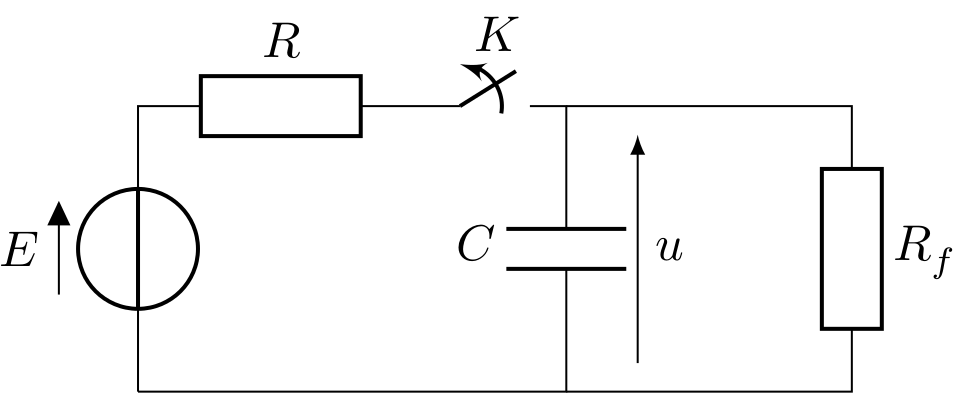
\includegraphics[width=\linewidth]{condo_fuite-plain}
		\end{center}
	\end{minipage}

	À $t = 0$, on ouvre le circuit. Au bout d’un temps $T > 0$, la valeur mesurée de
	$u$ est $E' < E$.
}%

\QR{%
	Comment peut-on expliquer ces observations~?
}{%
	En ouvrant le circuit, sans
	la résistance de fuite on s'attend à ce que le condensateur reste chargé,
	comme une pile. Or dans ce circuit, en ouvrant l'interrupteur la capacité
	$C$ est reliée à la résistance $R_f$ dans laquelle elle se décharge donc, ce
	qui explique la diminution de la tension.
}%

\QR{%
	Donner l'expression de $R_f$ en fonction de $C$, $E$, $E'$ et $T$. Faire
	l'application numérique pour $C = \SI{100}{pF}$, $T = \SI{2}{min}$, $E =
		\SI{10}{V}$ et $E' = \SI{1}{V}$.
}{%
	On a la situation de décharge du cours, où l'équation différentielle sur $u$ est
	\[ \dv{u_C}{t} + \frac{u_C}{R_f C} = 0\]
	Sachant que $u_C(t=0) = E$, la solution s'écrit
	\[\boxed{u_C(t) = E\exp \left( - \frac{t}{R_fC} \right)}\]
	Pour que $u_C(T) = E'$, il faut donc $\exp \left( - \frac{T}{R_fC} \right) =
		\frac{E'}{E}$, et finalement
	\[\boxed{R_f = \frac{T}{C\ln \frac{E}{E'}}} \qqdc \boxed{R_f \approx
			\SI{5.0e11}{\ohm}}\]
}%

\end{document}
